\documentclass{article}
\usepackage{amsmath}
\usepackage{tikz}
\usetikzlibrary{arrows.meta}

\begin{document}

\begin{figure}[h]
    \centering
    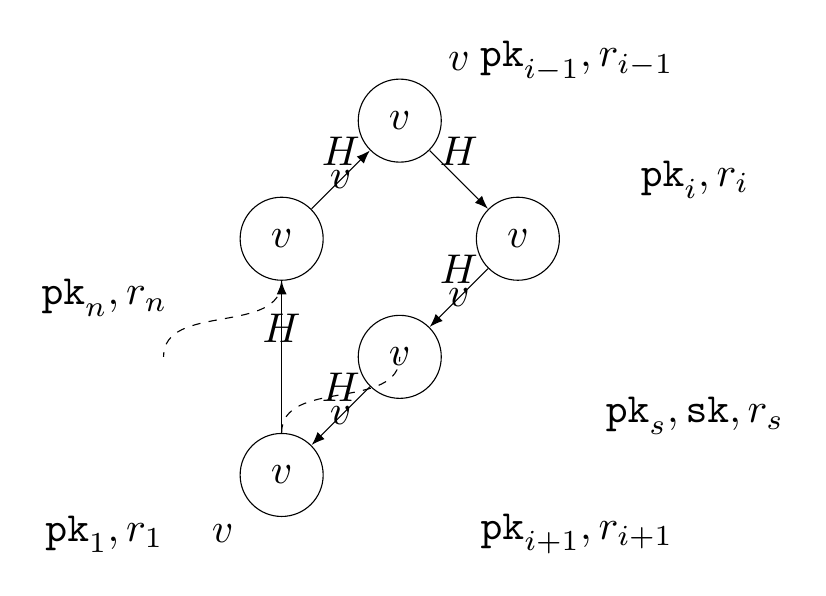
\begin{tikzpicture}[scale=1.5, transform shape]
        % Define styles for nodes and edges
        \tikzstyle{vertex}=[circle, draw, fill=white!20, minimum size=20pt, inner sep=0pt]
        \tikzstyle{edge} = [draw, -Latex]

        % Draw vertices
        \node[vertex] (v1) at (0, 0) {$v$};
        \node[vertex] (v2) at (1, 1) {$v$};
        \node[vertex] (v3) at (2, 0) {$v$};
        \node[vertex] (v4) at (1, -1) {$v$};
        \node[vertex] (v5) at (0, -2) {$v$};

        % Draw edges with labels
        \draw[edge] (v1) -- node[above] {$H$} (v2);
        \draw[edge] (v2) -- node[above] {$H$} (v3);
        \draw[edge] (v3) -- node[above] {$H$} (v4);
        \draw[edge] (v4) -- node[above] {$H$} (v5);
        \draw[edge] (v5) -- node[above] {$H$} (v1);

        % Draw dashed edges
        \draw[dashed] (v1) to[out=-90,in=90] ++(-1,-1);
        \draw[dashed] (v5) to[out=90,in=-90] ++(1,1);

        % Add labels for public keys and randomness
        \node at (-1.5, -0.5) {$\texttt{pk}_{n}, r_{n}$};
        \node at (2.5, 1.5) {$\texttt{pk}_{i-1}, r_{i-1}$};
        \node at (3.5, 0.5) {$\texttt{pk}_{i}, r_{i}$};
        \node at (3.5, -1.5) {$\texttt{pk}_{s}, \texttt{sk}, r_{s}$};
        \node at (2.5, -2.5) {$\texttt{pk}_{i+1}, r_{i+1}$};
        \node at (-1.5, -2.5) {$\texttt{pk}_{1}, r_{1}$};

        % Add labels for the commitment function
        \node at (0.5, 0.5) {$v$};
        \node at (1.5, 1.5) {$v$};
        \node at (1.5, -0.5) {$v$};
        \node at (0.5, -1.5) {$v$};
        \node at (-0.5, -2.5) {$v$};
    \end{tikzpicture}
    \caption{The Type-T structure of a ring signature as defined by the generic AOS ring signatures schemes \cite{abe2002}. In the figure, \( H \) corresponds to a collision-resistant hash function, \( v \) is a cryptographic commitment function and the \( r_i \)s and \( \mathsf{pk}_i \)s for \( 1 \leq i \leq n \) are unique randomness inputs and public keys respectively.}
    \label{fig:ring_signature_structure}
\end{figure}

\end{document}